%----------------------------------------------------------------------------------------
%       CHAPTER 16
%----------------------------------------------------------------------------------------

\cleardoublepage

\chapterimage{chx-plotting.png} % Chapter heading image

\chapter{muffinplot}\label{ch:muffinplot}

\hfill \break

%------------------------------------------------
\newpage
%------------------------------------------------

\noindent The \textbf{muffinplot} suite of \textbf{MATLAB} functions provides a means of plotting a variety of output reproducibly (by means of  a saved parameter file) and with the potential for automation (i.e. automatically generating the same analysis for a large number of different experiments).

The functions comprising this software suite include:

\begin{itemize}[noitemsep]
\vspace{1mm}
\item \footnotesize\textsf{plot\_fields\_biogem\_2d}\normalsize -- lon-lat plots from the 2D \textbf{biogem} output.
\vspace{1mm}
\item \footnotesize\textsf{plot\_fields\_biogem\_3d\_i}\normalsize -- lat-depth plots from the 3D \textbf{biogem} output.
\vspace{1mm}
\item \footnotesize\textsf{plot\_fields\_biogem\_3d\_k}\normalsize -- lon-lat plots from the 3D \textbf{biogem} output.
\vspace{1mm}
\item \footnotesize\textsf{plot\_fields\_ccd}\normalsize -- analsysis of the 'CCD' (from both \textbf{biogem} 2D and \textbf{sedgem} 2D output).
\vspace{1mm}
\item \footnotesize\textsf{plot\_fields\_sedgem\_2d}\normalsize -- lon-lat plots from the 2D \textbf{sedgem} output.
\vspace{1mm}
\item \footnotesize\textsf{plot\_histc\_2d}\normalsize -- a generic color-coded histogram function.
\vspace{1mm}
\item \footnotesize\textsf{plot\_sedcore}\normalsize -- down-core plots from \textbf{sedgem} sedcore output.
\vspace{1mm}
\item \footnotesize\textsf{plot\_timeseries\_biogem}\normalsize -- time-series plots from \textbf{biogem} time-series output.
\end{itemize}
Note that at this current time, there is no facility for lon-depth plotting (unlike in \textbf{Panoply}).

Most of the plots also perform additional functions (which can be generally disabled if not wanted), such as plotting and saving zonal or depth profiles, plotting difference maps, plotting and labelling data on maps and carrying out model-data fit statistics and plotting, extracting model values at data locations.

The following sections provide an overview and examples of such plotting and analysis.

%------------------------------------------------

\section{Installation}

\textbf{muffinplot} can be obtained from \href{https://github.com/derpycode/muffinplot\#https://github.com/derpycode/muffinplot}{github}. If you do not have a \textbf{git} client on your computer (and hence cannot clone the repository locally), then simply download the archive file of all the code (from \footnotesize\textsf{\textcolor[rgb]{0,0.501961,0}{clone or download }}\normalsize -- pick \textsf{\footnotesize Download ZIP}).

When you unpack (or clone) \textbf{muffinplot} (note that it is likely to unpack by default into its own directory), you should see 3 directories -- \footnotesize\textsf{EXAMPLES}\normalsize, and \footnotesize\textsf{MASKS}\normalsize,\ \footnotesize\textsf{source}\normalsize, a series of \footnotesize\textsf{.m }\normalsize files, and a single lonely \footnotesize\textsf{.ps }\normalsize graphics file (\footnotesize\textsf{colorscales.ps}\normalsize). The \footnotesize\textsf{.m }\normalsize files are split into filenames with or without the label \footnotesize\textsf{SETTINGS }\normalsize -- the ones without are code files (\textit{functions}), and the ones with the word \footnotesize\textsf{SETTINGS }\normalsize in their filename, contain parameter settings for plotting.

By default (the parameters can be changed if you wish), wherever you run the \textbf{muffinplot} plotting function from, requires that you also have a subdirectory called \footnotesize\textsf{cgenie\_output}\normalsize\ present, and that the (complete) \textbf{muffin} experiment output directories of anything you want to plot should be in subdirectories of that -- i.e. the contents of \footnotesize\textsf{cgenie\_output }\normalsize should look like the contents of \footnotesize\textsf{cgenie\_output }\normalsize on your cluster account\footnote{Although you do not need to copy \uline{all} the results over ... just the experiments that you wish to plot up.}. Mask files reside in the \footnotesize\textsf{MASKS}\normalsize\ subdirectory of the \textbf{muffinplot} installation, or in your current directory, or anywhere in the \textbf{MATLAB} path.

The simplest option is to unpack/clone \textbf{muffinplot} to a directory containing \footnotesize\textsf{cgenie\_output }\normalsize and hence all your experimental results directories.\footnote{However, the \textbf{muffinplot} functions do not have to be run from the same directory that you are in -- you can install them somewhere convenient, and then with \textbf{MATLAB} set to a directory containing a \textsf{cgenie\_output} experiment results directory, you can:
\\\texttt{>> addpath(PATH)}
\\where \texttt{PATH} is the path to the directory where \textbf{muffinplot} is installed.}
In other words:
\begin{enumerate}[noitemsep]
\vspace{1mm}
\item Create some local directory e.g. called \footnotesize\textsf{RESULTS}\normalsize.
\vspace{1mm}
\item Create a subdirectory in \footnotesize\textsf{RESULTS }\normalsize called \footnotesize\textsf{cgenie\_output}\normalsize.
\vspace{1mm}
\item Drag your experiment results folders across into the subdirectory \footnotesize\textsf{cgenie\_output}\normalsize, as per the directory structure on the cluster. (Or better -- drag the archived files to  \footnotesize\textsf{cgenie\_output }\normalsize and unpack them.)
\vspace{1mm}
\item Install \textbf{muffinplot} in the \footnotesize\textsf{RESULTS }\normalsize directory.
\vspace{1mm}
\item Change the \textbf{MATLAB} working directory to \footnotesize\textsf{RESULTS}\normalsize.
\end{enumerate}
\vspace{2mm}

The plotting functions are run simply by typing their name and passing a list of parameters (comma-separated, with the complete list enclosed in parentheses). By default,   the \footnotesize\textsf{SETTINGS }\normalsize files need to be in the same directory as you are running the functions from, or in one of the \textbf{MATLAB} paths. Results are saved to a subdirectory that by default is called \footnotesize\textsf{PLOTS}\normalsize, which will be created for you if it does not already exist.

All the plotting functions provide some manner of 'help', that can be obtained by typing at the command line:
\vspace{-2pt}\begin{verbatim}
>> help FUNCTIONNAME
\end{verbatim}\vspace{-2pt}
where \texttt{FUNCTIONNAME} is the function name (as per listed above).

%------------------------------------------------

\newpage 
\section{Time-series plotting}

The \textbf{muffinplot} function \textsf{\footnotesize plot\_timeseries\_biogem.m} provides a facility to plot \textbf{BIOGEM} \textit{time-series} (\textsf{\small .res}) output.\footnote{Obviously -- there are lots of different and easy ways of plotting plain text output in the form of a simple column format.} You can use \textbf{MATLAB} \texttt{help} on the function name to detail the parameters that need to be passed (and examples).

The \textsf{\footnotesize plot\_timeseries\_biogem} plotting function plots a basic set of time-series variables by default. It then, enables a set up up to 3 additional variables to be plotted. It is also associated with a file of parameter values (\textsf{\footnotesize plot\_timeseries\_SETTINGS.m} by default) for fine-tuning plots.

The plotting function requires a list of parameters to be passed in the argument list, i.e.:
\begin{verbatim}
>> plot_timeseries_biogem(PAR1,PAR2,PAR3, ... PARn)
\end{verbatim}

These are, in order:

\vspace{1mm}
\begin{enumerate}
\item \texttt{PEXP1} -- \textit{string} \(\rightarrow\) the (first) experiment name.
\item \texttt{PEXP2} -- \textit{string} \(\rightarrow\)  is the name of the 2nd (optional) experiment. If no second experiment is selected, then a null string value must be passed, i.e., \texttt{''}.
\item \texttt{PTMIN} -- \textit{real} \(\rightarrow\) minimum plotted time (\textit{x}-axis).
\item \texttt{PTMAX} -- \textit{real} \(\rightarrow\) maximum plotted time (\textit{x}-axis).
\item \texttt{PDATA1} -- \textit{string} \(\rightarrow\) time-series variable name for additional data to plot.
\\Omit the '\texttt{biogem\_series\_}' and '\texttt{.res}' parts of the filename.
\\Leave blank, i.e., '', for no additional data panel.
\item \texttt{PDATA1N} -- \textit{integer} \(\rightarrow\) the column number of the data in the time-series file.
\item \texttt{PDATA2} -- \textit{string} \(\rightarrow\) time-series variable name for additional data to plot.
\item \texttt{PDATA2N} -- \textit{integer} \(\rightarrow\) the column number of the data in the time-series file.
\item \texttt{PDATA3} -- \textit{string} \(\rightarrow\) time-series variable name for additional data to plot.
\item \texttt{PDATA3N} -- \textit{integer} \(\rightarrow\) the column number of the data in the time-series file.
\item \texttt{POPT} -- \textit{string}\(\rightarrow\) The string for an alternative plotting parameter set.
\\If an empty\texttt{ ('') }value is passed as this parameter, then the default parameter set file is used.
\item \texttt{PNAME}  -- \textit{string}\(\rightarrow\) The string for an alternative filename.
\end{enumerate}
\vspace{2mm}
Note that if an empty value is passed as this parameter, then a filename is automatically generated.

A simple example usage would be:

\begin{verbatim}
>> plot_timeseries_biogem('myexperiment','',0.0,10000.0,'',0,'',0,'',0,'','')
\end{verbatim}
where \texttt{myexperiment} is the name of the 1st experiment, followed by and empty string (\texttt{''}) indicating no second experiment. The results are to be plotted from 0.0 to 10000.0 years (the 2 following parameters; \texttt{0.0,10000.0}). Then, no additional (maximum 3) optional parameters are requested, and hence the next parameters passed are: \texttt{'',0,'',0,'',0}. Finally, the default plotting parameter set is required, and no specific alternative filename is ot be used, accounting for the final 2 empty strings passed.

By default, \textsf{\footnotesize plot\_timeseries\_biogem} plots 2 panels of data, both with 2 (LH\ and RH) axes:

\begin{enumerate}[noitemsep]
\vspace{1mm}
\item Atmospheric \(CO_{2}\). Note that if the experiment was not \(CO_{2}\)-enabled (i.e. not run with a global carbon cycle), a warning is given and 'fake' data (actually, random numbers) is plotted.
\vspace{1mm}
\item Atmospheric \(\delta ^{13}CO_{2}\). Note that if the experiment was not \(\delta ^{13}CO_{2}\)-enabled (i.e. not run with a global carbon cycle), a warning is given and 'fake' data is plotted.
\vspace{1mm}
\item Atmospheric temperature (as a global mean, annual average).
\vspace{1mm}
\item Fractional (percentage) sea-ice extent.
\end{enumerate}
\vspace{2mm}

Additional model outputs can then be added by listing them in the function call. For example, to also plot the global overturning strength, which is contained in the file \footnotesize\textsf{biogem\_series\_misc\_opsi.res}\normalsize, you would add \texttt{'misc\_opsi',3}\footnote{Don't forget that you omit the '\texttt{biogem\_series\_}' and '\texttt{.res}' parts of the filename.}, where the \texttt{3} indicates the 3rd column of data in the file is to be plotted, which in this case is the global maximum overturning value (and the 2nd column is the minimum value). The complete line looks like:
\small\begin{verbatim}
>> plot_timeseries_biogem('myexperiment','',0.0,10000.0,'misc_opsi',3,'',0,'',0,'','')
\end{verbatim}\normalsize

By default, the plotted variables are all auto-scaled. To specify the y-axes, you will need to edit the plotting settings parameter file: \footnotesize\textsf{plot\_timeseries\_SETTINGS.m}\normalsize. For the default plotted 4 results variables, the minimum and maximum y-axis limits are specified in the section:
\vspace{1mm}
\begin{itemize}
\item[] \texttt{axis\_pCO2min = 0.0;}
\item[] \texttt{axis\_pCO2max = 0.0;}
\item[] \texttt{axis\_d13Cmin = 0.0;}
\item[] \texttt{axis\_d13Cmin = 0.0;}
\item[] \texttt{axis\_Tatmmin = 0.0;}
\item[] \texttt{axis\_Tatmmin = 0.0;}
\item[] \texttt{axis\_icemin = 0.0;}
\item[] \texttt{axis\_icemin = 0.0;}
\end{itemize}
\vspace{2mm}
The default zero values here, tell the plotting function to create an auto-scale for the y-axis.\footnote{Note the units of atmospheric \(CO_{2}\) as \(\mu atm\).} Following this in the parameter file, are the settings for the optional variable plotting:
\vspace{1mm}
\begin{itemize}
\item[] \texttt{axis\_data1\_min = 0.0;}
\item[] \texttt{axis\_data1\_max = 0.0;}
\item[] \texttt{axis\_data2\_min = 0.0;}
\item[] \texttt{axis\_data2\_max = 0.0;}
\item[] \texttt{axis\_data2\_min = 0.0;}
\item[] \texttt{axis\_data2\_max = 0.0;}
\end{itemize}
\vspace{2mm}

Note that if you want instead to copy and rename and then edit this settings file, you will need to pass the new (non-default) filename when calling the plotting function. For example, if you created a new parameter settings file: \footnotesize\textsf{settings\_NEW.m }\normalsize, then the \textit{function} call would look like:
\small\begin{verbatim}
>> plot_timeseries_biogem('myexperiment','',0.0,10000.0,'',0,'',0,'',0,'settings_NEW','')
\end{verbatim}\normalsize

%------------------------------------------------

\section{Spatial plotting}

%------------------------------------------------

\subsubsection{Overview}

4 of the \textbf{muffinplot} plotting functions provide spatial (2D) plotting capabilities:
\vspace{2mm}
\begin{itemize}

\item \texttt{plot\_fields\_biogem\_2d}
\\Plot a 2-D field from: \footnotesize\textsf{fields\_biogem\_2d.nc}\normalsize.

\item \texttt{plot\_fields\_biogem\_3d\_i}
\\Plot a vertical-meridional (2-D) slice through the ocean (i.e., all cells have the same \texttt{i} (longitudinal) coordinate value) from: \footnotesize\textsf{fields\_biogem\_3d.nc}\normalsize.
\\Options are  provided for averaging longitudinally over a supplied mask, which may be the entire ocean and hence giving a global meridional cross-sectional mean, of a specific ocean basin, or may be a single cell 'wide' longitudinally and take a meandering path hence simulating an ocean transect. An option is also provided to overlay an ocean circulation stream-function.

\item \texttt{plot\_fields\_biogem\_3d\_k.m}
\\Plot a horizontal slice through the ocean from: \footnotesize\textsf{fields\_biogem\_3d.nc}\normalsize.
\\An option is provided for overlaying ocean circulation (velocity fields). Water column integrals  can also be calculated and displayed, as well as benthic surfaces, and the function can also determine the spatial distribution of the maximum or minimum value occurring anywhere in the water column (or portion of the water column).

\item \texttt{plot\_fields\_sedgem\_2d}
\\Plot a 2-D field from: \texttt{fields\_sedgem\_2d.nc}.

\end{itemize}
\vspace{2mm}

All 4 plotting functions can also overlay observed data and create difference (anomaly) maps -- either between different experiments, time-slices, or variables, or between model and data and provide summary statistics regarding the difference.

\subsubsection{Argument (parameter) list}

All 4 plotting functions share exactly the same format of parameters\footnote{Parameters can be in for form of strings, in which case they must be given as a series of characters enclosed in inverted commas \texttt{''}; as real numbers, e.g. \texttt{999.5} or \texttt{9.995E2}; or integers, e.g. \texttt{2}, \texttt{10}.} passed in the argument list:

\vspace{-2mm}
\small\begin{verbatim}
>> FUNCTIONNAME(PAR1,PAR2,PAR3, ... PARn)
\end{verbatim}\normalsize
\vspace{-2mm}
\noindent i.e. take a (long!) list of parameters. These are (in order):

\vspace{1mm}
\noindent Firstly, a series of parameters for defining experiment, variable, and year:

\vspace{1mm}
\begin{enumerate}
\item \texttt{PEXP1} -- \textit{string} -- is the name of the 1st (main) experiment. A results directory with the same name must exist in the directory \footnotesize\textsf{cgenie\_output}\normalsize\footnote{Or alternative directory if the default file path settings have been changed.}.
\item \texttt{PEXP2} -- \textit{string} -- is the name of the 2nd (optional) experiment. If no second experiment is selected, then a null string value must be passed, i.e., \texttt{''}.
\item \texttt{PVAR1} -- \textit{string} -- is the name of the 1st (main) variable. If no valid variable value is given, a list of valid variable names will be printed out.\footnote{As a string, the value must be encased in inverted commas: \texttt{''}.}
\item \texttt{PVAR2} -- \textit{string} -- is the name of the 2nd (optional) variable. If no second variable is selected, then a null string value must be passed, i.e., \texttt{''}.
\item \texttt{PT1} -- \textit{real} (or \textit{integer}) -- is the value of the 1st (main) time-slice. If no valid variable value is given, a list of valid variable names will be printed out.\footnote{As \textbf{sedgem} does not save multiple and/or time-specific data, a dummy value (anything) is entered here.}
\item \texttt{PT2} -- \textit{real} (or \textit{integer}) -- is the value of the 2nd (optional) time-slice. If no second time-slice is selected, then enter \texttt{-1}.\footnote{As \textbf{sedgem} does not save multiple and/or time-specific data, a dummy value (anything) is entered here.}
\end{enumerate}
\vspace{1mm}

Then there are 2 parameters for plotting sub-sets of the 2D or 3D data (essential for 3D data which cannot be usefully visualized in raw form):

\vspace{1mm}
\begin{enumerate}
\item \texttt{PIK} -- \textit{integer} -- varies in its interpretation and is discussed below.
\item \texttt{PMASK} -- \textit{string} -- is the name of an optional (2D) mask. A null string (\texttt{''}) must be passed if no mask is requested. A file with the same name (plus an extension \footnotesize\textsf{.dat}\normalsize) must exist in the directory \footnotesize\textsf{MASKS}\normalsize\footnote{Or alternative directory if the default file path settings have been changed.}. The interpretation of this parameter differs slightly between functions (below).
\end{enumerate}
\vspace{1mm}

Next come options for plotting scale control:

\vspace{1mm}
\begin{enumerate}
\item \texttt{PCSCALE} -- \textit{real} (or \textit{integer}) -- is the scale factor for the plot. For example, to plot in micro molar (umol kg-1) units, enter; \texttt{1e-6}. The plot is auto-scaled if a value of zero (\texttt{0.0}) is entered.
\item \texttt{PCMIN} -- \textit{real} (or \textit{integer}) -- is the minimum scale value.
\item \texttt{PCMAX} -- \textit{real} (or \textit{integer}) -- is the maximum scale value.
\item \texttt{PCN} -- \textit{integer} -- is the number of (contour) intervals between minimum and maximum scale values.
\end{enumerate}
\vspace{1mm}

Finally, there are 3 parameters for: specifying discrete (observed) data to be plotted (and analyzed against model projections), for specifying the plotting parameter file to be used, and for substituting an alternative filename for all the output:

\vspace{1mm}
\begin{enumerate}
\item \texttt{PDATA} -- \textit{string} -- is the filename containing the an overlay data set, which must be formatted as separated columns. The precise number and type of columns varies between different functions and also the plotting options chosen, and are hence discussed later. The full filename of this file must be give, \uline{including} any extensions (e.g. \footnotesize\textsf{.dat }\normalsize, \footnotesize\textsf{.txt}\normalsize). This parameter must be passed as a \textit{string}; leave blank, i.e., \texttt{''}, for no overlay data.
\item \texttt{POPT} -- \textit{string} -- is the \footnotesize\textsf{m-file }\normalsize filename (excluding the \footnotesize\textsf{.m }\normalsize extension) containing the plotting options (\footnotesize\textsf{SETTINGS}\normalsize). This parameter must be passed as a string; leave blank, i.e., \texttt{''}, in order to load the default file (\footnotesize\textsf{plot\_fields\_SETTINGS}\normalsize).
\item \texttt{PNAME} -- \textit{string} -- is the string for an alternative series of output filenames. This parameter must be passed as a string, e.g., \texttt{'experiment2'}. If an empty (i.e., \texttt{''}) value is passed to this parameter then the output filenames will be automatically generated.
\end{enumerate}
\vspace{1mm}

\vspace{1mm}
The basic parameter list for all 4 plotting functions\footnote{Note that for \texttt{plot\_fields\_sedgem\_2d} several of the parameters are redundant but \uline{must} still be included (typically as zeros). This is in order to retain a common parameter list format between all the different plotting functions.} is hence:
\footnotesize
\vspace{-4pt}\begin{verbatim}
>> FUNCTIONNAME(PEXP1,PEXP2,PVAR1,PVAR2,PT1,PT2,PIK,PMASK,PCSCALE,PCMIN,PCMAX,PCN,PDATA,POPT,PNAME);
\end{verbatim}\vspace{-4pt}
\normalsize

\subsubsection{Function specific interpretation of PIK and PMASK}

A note on the different behaviour of 2 of the passed parameters, depending on whcih plotting function is used -- \texttt{PIK}, and to some extent, \texttt{PMASK}, have quite different interpretations depending on the particular plotting function used:

\begin{enumerate}

\vspace{2pt}
\item \texttt{plot\_fields\_biogem\_2d}
\begin{enumerate}
\vspace{1pt}
\item \texttt{PIK} -- is the maximum depth (\texttt{k}) level that will be plotted, i.e. all depth levels deeper than \texttt{PIK} will be excluded. This is useful for plotting a variable only for the 'deep' ocean (rather than the ocean overlaying all ocean depths) for example. This value also provides an alternative way of creating a mask, and only values of \texttt{k} less than of equal to the passed value will be plotted.
\vspace{1pt}
\item \texttt{PMASK} -- is the name of an optional (2D) mask. A null string (\texttt{''}) must be passed if no mask is requested. (Shallow depths could also be excluded from the plot by means of a mask rather than setting \texttt{PIK}.)
\end{enumerate}

\vspace{2pt}
\item \texttt{plot\_fields\_biogem\_3d\_k}
\begin{enumerate}
\vspace{1pt}
\item \texttt{PIK} -- the depth (\texttt{k}) level to be plotted. Note that the levels are numbered from a maximum value designating the surface, to 1 for the deepest ocean level. Typically, maximum values for the number of ocean levels are \texttt{8} (e.g. \textit{Ridgwell et al.} [2007]) or \texttt{16} (e.g. \textit{Cao et al.} [2009]).
\\Non ocean level \texttt{k} values have special meanings here:
\begin{enumerate}[noitemsep]
\vspace{1pt}
\item \texttt{0}
\\A zero will result in a water column integral being plotted. With data, the model-data is  carried out on the grid as a whole.
\vspace{1pt}
\item \texttt{-1}
\\Will result in the benthic surface being plotted.
\end{enumerate}
\vspace{1pt}
\item \texttt{MASK} -- is the name of an optional (2D) mask. A null string (\texttt{''}) must be passed if no mask is requested.
\end{enumerate}

\vspace{2pt}
\item \texttt{plot\_fields\_biogem\_3d\_i}
\begin{enumerate}
\vspace{1pt}
\item \texttt{PIK} -- the longitude-depth (\texttt{i}) slice through the ocean to be plotted.
\\Non longitude grid point \texttt{i} values have special meanings here:
\begin{enumerate}[noitemsep]
\vspace{1pt}
\item \texttt{0}
\\A zero will result in a zonal mean being plotted. With data, model-data comparison is conducted at the specific data locations, rather than vs. a zonal mean model value.
\vspace{1pt}
\item \texttt{-1}
\\I have forgotten what this does ...
\end{enumerate}
\vspace{1pt}
\item \texttt{MASK} -- is the name of an optional (2D) mask. A null string (\texttt{''}) must be passed if no mask is requested.
\\ For example: if the mask is of the entire ocean (\texttt{mask\_worbe2\_ALL.dat}), the result is a global meridional cross-sectional mean.
\\ If the mask is just of a single basin such as the Atlantic (\texttt{mask\_worjh2\_Atlantic.dat}), the result is the Atlantic meridional cross-sectional mean.
\\ Masks can also be constructed that are only a single cell wide longitudinally, but which take a meandering path following an ocean transect\footnote{e.g., as in: \textsf{mask\_worjh2\_GEOSECS\_WATL.dat}}.
\\ The trivial usage would be to construct a mask consisting of a vertical line of \texttt{1}s -- the result is equivalent to setting an appropriate \texttt{i} value in \texttt{PIK}.
\end{enumerate}

\vspace{2pt}
\item \texttt{plot\_fields\_sedgem\_2d.m} is an exception as it does not (currently) use either parameter. \texttt{PIK} must be entered as \texttt{0} (any integer will do in fact), and \texttt{PMASK} as \texttt{''}.

\end{enumerate}
\vspace{4pt}

The mask itself (if \texttt{PMASK} contains a mask name) is a 2-D array of model grid points (on the \textbf{BIOGEM} grid) in the form of a simple ASCII file. A value of '\texttt{1}' represents a vertical column of ocean cells to include, whereas a value '\texttt{0}' will exclude all cells in the water column at that particular grid point. Examples of some masks can be found in the \footnotesize\textsf{MASKS }\normalsize subdirectory of \textbf{muffinplot}.

%------------------------------------------------
%
\pagebreak

\subsection{Basic usage}

What follows are some basic and quasi random examples, just to illustrate a simple use of the three main plotting functions.

\begin{enumerate}[noitemsep]

\vspace{4pt}
\item \textbf{Surface ocean temperature}

Surface ocean temperature can be plotted in 2 ways -- via the 2d plotting function (but only if the surface tracer properties fields have been saved, as these are optional), or via the 3d plotting function.

\begin{figure}[ht]
\begin{center}
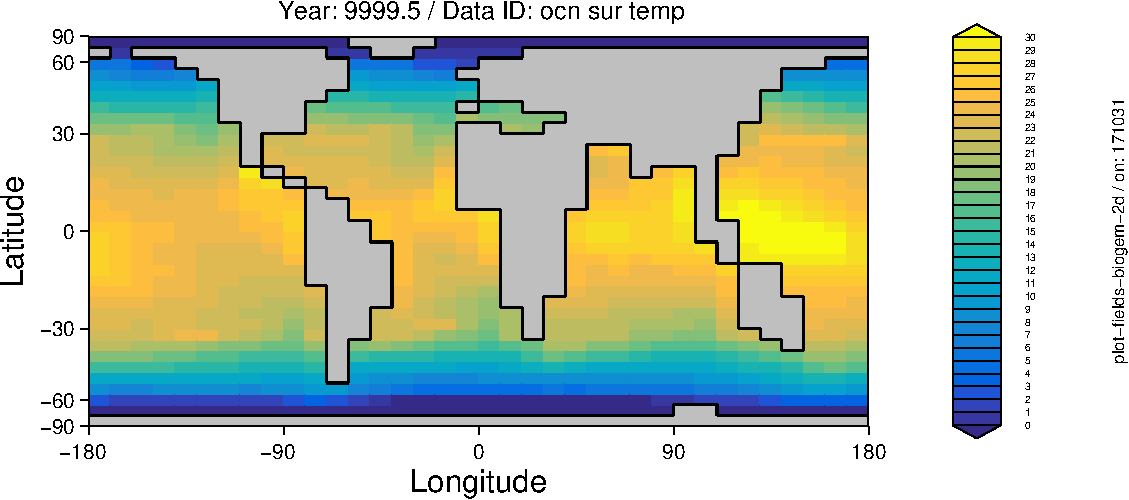
\includegraphics[scale=0.5]{example1a_171031.pdf}
\end{center}
\vspace{-4mm}
\caption{Example basic (default) surface temperature plot.}
\label{fig:example1a}
\end{figure}

For example:

\footnotesize
\vspace{-0pt}\begin{verbatim}
>> plot_fields_biogem_2d ...
('EXP1','','ocn_sur_temp','',9999.5,-1,16,'',1.0,0.0,30.0,30,'','','example1a');
\end{verbatim}\vspace{-0pt}
\normalsize
plots from the experiment \texttt{EXP1}, the variable \texttt{ocn\_sur\_temp} for time-slice \texttt{9999.5} (the mid-point time of the final year of a 10,000 year experiment). The color scale is from \texttt{0.0} to \texttt{30.0}, with no re-scaling (\texttt{1.0}), and \texttt{30} color intervals in the scale. The default \footnotesize\textsf{SETTINGS }\normalsize parameter file is used, and the default filename string replaced with \texttt{example1a}. The only other thing to note, is for parameter \texttt{PIK}, a value of \texttt{16} is set -- corresponding to the ocean surface. See Figure \ref{fig:example1a}.

Note that in this example, the   variable \texttt{ocn\_sur\_temp} is assumed. However, the model results variable \texttt{ocn\_sur\_temp} is not always saved in \textbf{BIOGEM} 2D netCDF output. If the requested variable, such as \texttt{ocn\_sur\_temp} does not exist, or is mis-spelt, \textbf{MATLAB} will pause and provide a warning. It will then list all the variables in the netCDF file that it can find and wait for a new variable name to be inputted. For instance, a variable that is always saved in \textbf{BIOGEM} 2D netCDF output is \texttt{atm\_temp} (surface air temperature) and could be substituted in the plot. Also note that time (the time-slice year to be plotted) is similarly handled -- if the specific time-slice value does not exist, a list of all possible time-slice years are provided and a substitute value requested as \textbf{MATLAB} pauses and wait for your input.

\begin{figure}[ht]
\begin{center}
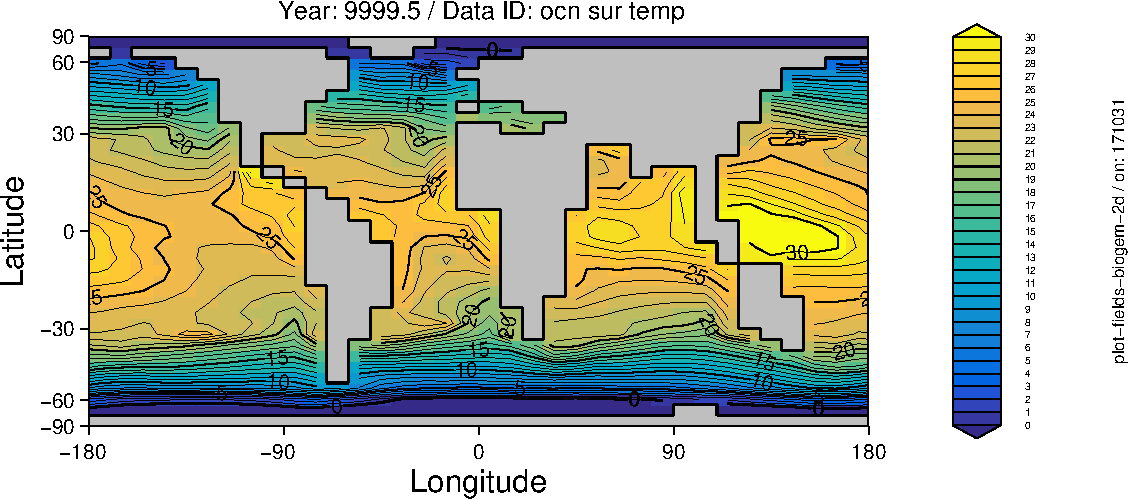
\includegraphics[scale=0.5]{example1b_171031.pdf}
\end{center}
\vspace{-4mm}
\caption{Example surface temperature plot, with contours.}
\label{fig:example1b}
\end{figure}

\vspace{4pt}
To add contours, in the default \footnotesize\textsf{SETTINGS }\normalsize parameter file (or a copied and re-named version thereof), adjust the following line:
\small
\vspace{-2pt}\begin{verbatim}
contour_plot = 'y';     % [ 'y']  OVERLAY CONTOUR PLOT?
\end{verbatim}\vspace{-2pt}
\normalsize
The results of this are shown in Figure \ref{fig:example1b}.

\pagebreak

Refinements to the contouring can be done by changing the lines:
\small
\vspace{-2pt}\begin{verbatim}
contour_mod = 1;        % [   1]  NUMBER OF COLOR INTERVALS PER CONTOR
contour_mod_label = 5;  % [   5]  NUMBER OF LABELED CONTOURS PER CONTOUR
contour_label = 'y';    % [ 'y']  LABEL CONTOURS?
contour_dashneg = 'n';  % [ 'n']  PLOT NEGATIVE CONTOURS DASHED?
\end{verbatim}\vspace{-2pt}
\normalsize
(these are the more commonly used refinements).

Here: \texttt{contour\_mod} determines how many color intervals per contour interval, which in the previous SST plot example, was \texttt{30}. So a value of \texttt{1} will give you 30 contours -- one every 1 degree C. And a value of \texttt{5} will give you 6 contours -- one each 5 degrees C.

\texttt{contour\_mod\_label} then determines whether you want the contours labelled or not. The answer (parameter value) to be the character \texttt{y} or \texttt{n}, as a string (i.e. in inverted commas). If you elect to have contour labels, \texttt{contour\_mod\_label} determines how frequently to label the contours. A value of \texttt{1} labels every single contour. A value of \texttt{2} labels every other contour. So for instance, if you set \texttt{contour\_mod=5} and \texttt{contour\_mod\_label=2} in the previous SST example, you get a contour every \texttt{5} degrees C, and a temperature label every \texttt{10} degrees C.

\vspace{4pt}
Alternatively, using 3d plotting, you could plot the ocean surface temperature field as follows:

\footnotesize
\vspace{-0pt}\begin{verbatim}
>> plot_fields_biogem_3d_k ...
('EXP1','','ocn_temp','',9999.5,-1,16,'',1.0,0.0,30.0,30,'','','example1c');
\end{verbatim}\vspace{-0pt}
\normalsize
The main things that change here are firstly the variable name -- now \texttt{ocn\_temp}, and secondly because this is a 3D ocean field, we need to specify what ocean model level we want to plot -- this is where the integer \texttt{16} comes in and corresponds to the input  \texttt{PIK}, as discussed earlier. The resulting plot will be identical to Figure \ref{fig:example1a}.

\vspace{4pt}
\item \textbf{Global zonal average temperature profile}

To keep with ocean temperature, we can use the \texttt{plot\_fields\_biogem\_3d\_i} function to plot the global zonal mean (lat-depth) profile (rather than horizontal, surface slice):

\footnotesize
\vspace{-0pt}\begin{verbatim}
>> plot_fields_biogem_3d_i ...
('EXP1','','ocn_temp','',9999.5,-1,0,'',1.0,0.0,30.0,30,'','','example2a');
\end{verbatim}\vspace{-0pt}
\normalsize
The only significant change as compared to before, is setting a \texttt{0} for input parameter \texttt{PIK} (again -- see earlier). The results is shown in Figure \ref{fig:example2a}.

\begin{figure}[ht]
\begin{center}
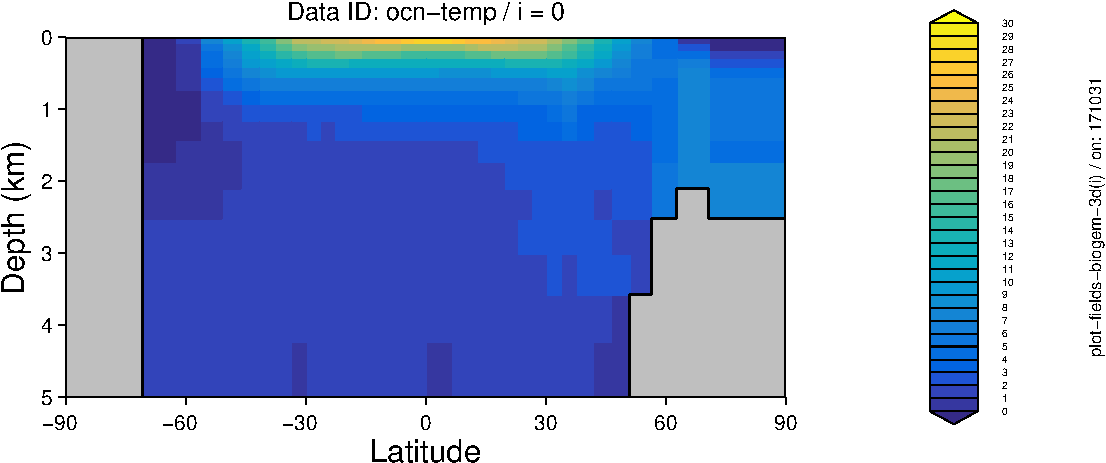
\includegraphics[scale=0.5]{example2a_171031.pdf}
\end{center}
\vspace{-4mm}
\caption{Zonal mean global ocean temperature profile.}
\label{fig:example2a}
\end{figure}

\vspace{4pt}
\item \textbf{Pacific dissolved oxygen profile}

As per choosing ocean levels (\texttt{k}-values) in the lon-lat plotting, you can also specify a specific longitude for creating a lat-depth section rather than calculating and plotting a global zonal mean. e.g. Figure \ref{fig:example3a} was created by\footnote{Also turning on the contour plotting.}:

\footnotesize
\vspace{-0pt}\begin{verbatim}
>> plot_fields_biogem_3d_i ...
('EXP1','','ocn_O2','',9999.5,-1,10,'',1.0E-6,0.0,300.0,30,'','','example3a');
\end{verbatim}\vspace{-0pt}
\normalsize
The chosen section is somewhere in the Pacific, along a line of longitude (whatever corresponds to \texttt{i=10} on this \textbf{muffin} model grid ... I guess about 165W ...). Here, the variable to be plotted has also been changed -- \texttt{ocn\_O2}\footnote{You'll need a biogeochemsitry enabled \textit{base-config}}. Because the units of dissolved oxygen are much smaller than for temperature (in degrees C),  the plotted scale has also been changed -- from 0 to 300 \(\mu mol kg^{-1}\) rather than the netCDF variable units of \(mol kg^{-1}\). To achieve this re-scaling, a units scaling value of \texttt{1.0E-6} is specified for parameter \texttt{PCSCALE}.\footnote{Note that the scaling specified is as the new units relative to the old units -- here, \(\mu mol kg^{-1}\) relative to \(mol kg^{-1}\) and hence \(10^{-6}\). ALSO NOTE that \textbf{Panoply} does it the other way around ... :(}

\begin{figure}[ht]
\begin{center}
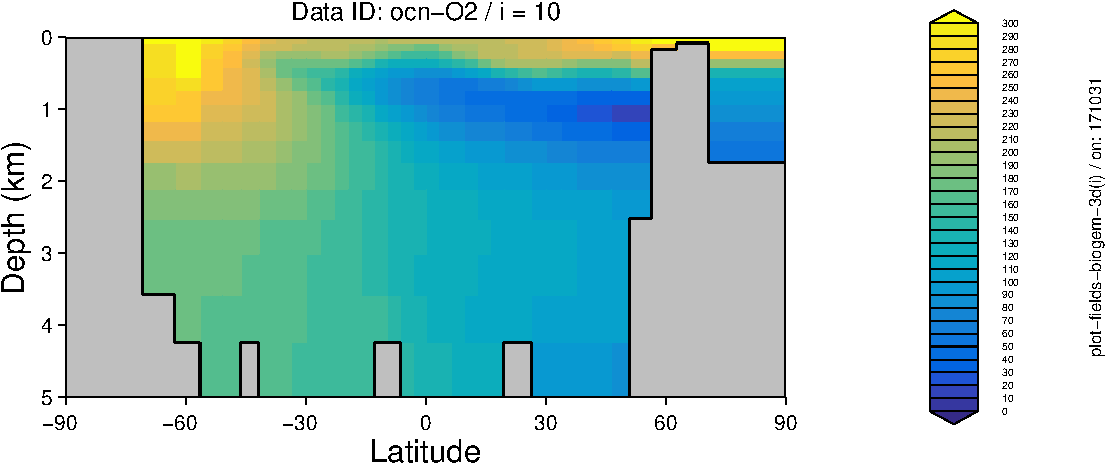
\includegraphics[scale=0.5]{example3a_171031.pdf}
\end{center}
\vspace{-4mm}
\caption{Ocean oxygen profile on a Pacific transect.}
\label{fig:example3a}
\end{figure}

\vspace{4pt}
\item \textbf{Atlantic zonal mean dissolved oxygen profile}

So far, with the exception of plotting a gridded color field \uline{and} a contoured field at the same time, all these examples can also be done in \textbf{Panoply}. One difference, is the ability in the \textbf{muffinplot} suite of \textbf{MATLAB} functions to apply masks -- isolating geographical regions or even single points. In the \footnotesize\textsf{MASKS }\normalsize directory, are a series of example ASCII mask files, mostly for the 2 (8- and 16-level ocean) modern published configurations of \textbf{muffin}. For instance, \footnotesize\textsf{mask\_worjh2\_AtlanticALL.dat }\normalsize has all the grid points in the entire Atlantic basin assigned a value of \texttt{1}, with \texttt{0} everywhere else. If we apply this first to the surface ocean dissolved oxygen field:

\footnotesize
\vspace{-0pt}\begin{verbatim}
>> plot_fields_biogem_3d_k ...
('EXP1','','ocn_O2','',9999.5,-1,16,'mask_worjh2_AtlanticALL.dat',1.0E-6,0.0,300.0,30,
... '','','example4a');
\end{verbatim}\vspace{-0pt}
\normalsize
we obtain Figure \ref{fig:example4a}.

\begin{figure}[ht]
\begin{center}
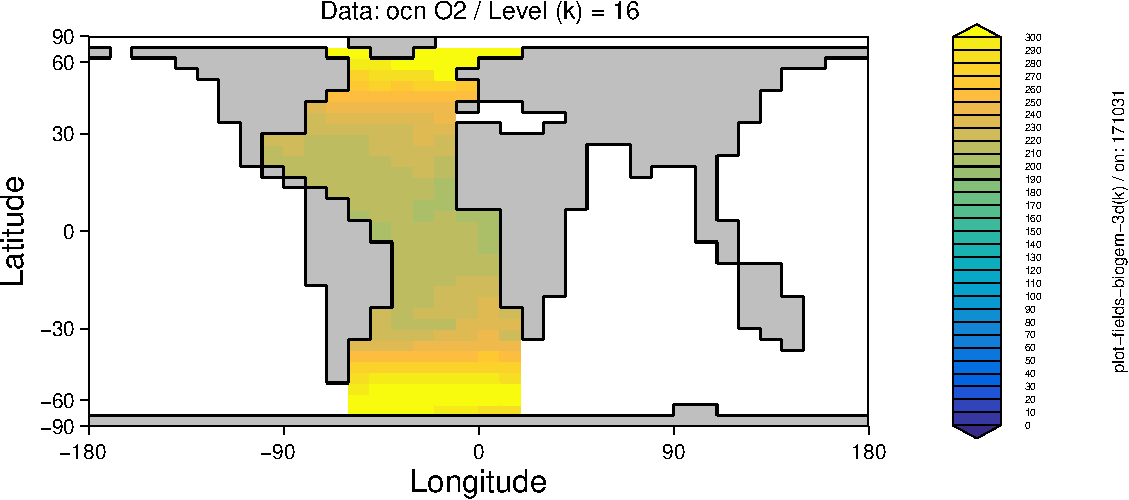
\includegraphics[scale=0.5]{example4a_171031.pdf}
\end{center}
\vspace{-4mm}
\caption{Distribution of surface ocean dissolved  oxygen in the Atlantic.}
\label{fig:example4a}
\end{figure}

Here, it is clear how the masked has been applied and all the ocean falling outside of the mask is plotted as white (no data).

We can also apply a mask field to the zonal average plot:

\footnotesize
\vspace{-0pt}\begin{verbatim}
>> plot_fields_biogem_3d_i ...
('EXP1','','ocn_O2','',9999.5,-1,0,'mask_worjh2_AtlanticALL.dat',1.0E-6,0.0,300.0,30,
... '','','example4b');
\end{verbatim}\vspace{-0pt}
\normalsize
(Figure \ref{fig:example4b})

\begin{figure}[ht]
\begin{center}
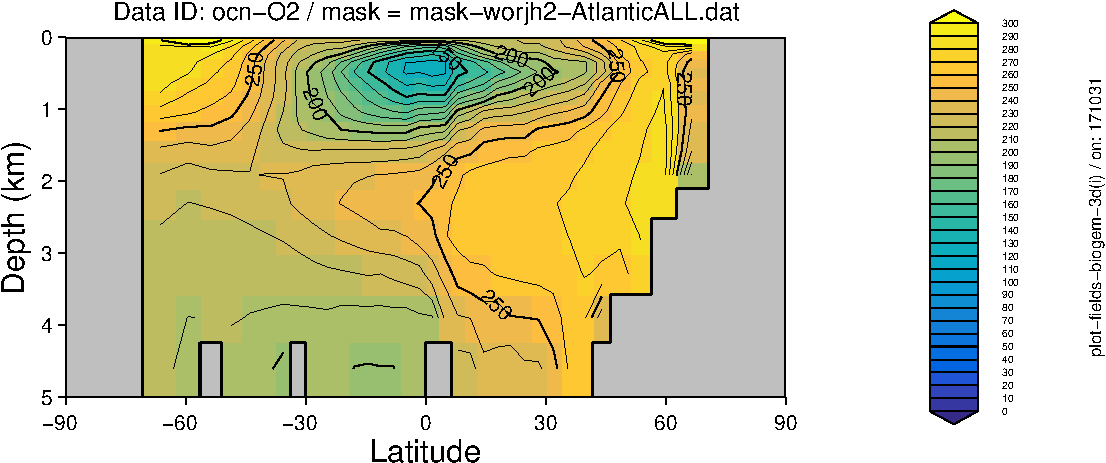
\includegraphics[scale=0.5]{example4b_171031.pdf}
\end{center}
\vspace{-4mm}
\caption{Mean zonal ocean oxygen profile in the Atlantic.}
\label{fig:example4b}
\end{figure}

\end{enumerate}

%------------------------------------------------

\subsection{Difference maps}



%------------------------------------------------

\subsection{Model-data and data maps}



%------------------------------------------------

\subsection{Example plotting suite}

An set of \textbf{MATLAB} \footnotesize\textsf{m-file }\normalsize functions are provided that define a series of different generic and basic experiment analysis and plottings, with \footnotesize\textsf{make\_analysis\_ALL.m }\normalsize provided as a template for carrying them all out in one go. Obviously, the individual aggregate plotting functions can be edited, added to, or with unwanted or irrelevant plots, commented out or deleted -- treat these all simply as templates for developing your own analysis strategy (as well as viewing the associated configuration files as illustrations of the function/use of some of the different further plotting options\footnote{Also covered in a subsequent sub-sub-section.}).

The aggregate plotting functions are as follows:

\begin{enumerate}[noitemsep]

\vspace{1pt}
\item \footnotesize\textbf{\textsf{fun\_make\_analysis\_phys.m}}\normalsize \\This encompasses a basic set of analyses of ocean circulation and climatology.
\\The script is written as a \textit{function}, and requires just two parameters to be passed as input:
\begin{enumerate}[noitemsep]
\setlength{\itemindent}{.2in}
\item The experiment name.
\item The (mid-point of the) year of the time-slice to plot.
\end{enumerate}
In the example of an experiment called \texttt{'EXP1'}, and plotting the last annual time-slice (\texttt{9999.5}) from a 10,000 year model run, the function is hence called:
\vspace{-2pt}\begin{verbatim}
fun_make_analysis_phys('EXP1',9999.5);
\end{verbatim}\vspace{-2pt}

\vspace{1pt}
\item \footnotesize\textbf{\textsf{fun\_make\_analysis\_geo.m}}\normalsize \\This encompasses a basic set of analyses of ocean (abiotic) geochemistry and ocean acidification related variables and metrics.

\vspace{1pt}
\item \footnotesize\textbf{\textsf{fun\_make\_analysis\_bio.m}}\normalsize \\This encompasses a basic set of analyses of marine biological fluxes and biologically related properties.

\vspace{1pt}
\item \footnotesize\textbf{\textsf{fun\_make\_analysis\_ALL.m}}\normalsize
\\Aggregates all the above functions (i.e., calls all 3).
\end{enumerate}

\vspace{2pt}
To run these example analysis -- either copy all the files contained in the \footnotesize\textsf{EXAMPLES }\normalsize subdirectory, to your working directory (e.g. \footnotesize\textsf{RESULTS }\normalsize as per the previous example). Then type e.g..\footnote{Note that if you did not run with ocean biogeochemsitry (but rather climate-only), not all the plotting functions will run and you will have to restrict this default analysis to: \texttt{fun\_make\_analysis\_phys('EXP1',9999.5);}}

\vspace{-2pt}\begin{verbatim}
fun_make_analysis_ALL('EXP1',9999.5);
\end{verbatim}\vspace{-2pt}

\noindent OR, add the path to the \footnotesize\textsf{EXAMPLES }\normalsize subdirectory, e.g.
\vspace{-2pt}\begin{verbatim}
addpath('Y:\_git\muffinplot\EXAMPLES');
\end{verbatim}\vspace{-2pt}
but obviously depending on quite where you installed \textbf{muffinplot}.

%------------------------------------------------

\subsection{Further refinements}

A number of additional options for exerting finer control over the plotting are provided as a block of parameters and (default) values in the m-file itself, in a section immediately after the commented help and change-log at the start of the m-file. Not all the options are relevant to all the plotting functions\footnote{See 'help' on a specific plotting function for details of the relevant options in the parameter block.}, but the full list (and then defaults in brackets \texttt{[]}) is as follows:

\vspace{2pt}
{\small \begin{enumerate}
\item \texttt{lon\_min = -180;         [-180]  STARTING LONGITUDE FOR X-AXIS}
\\ Sets the longitude of the left-hand edge of the plot.
\item \texttt{delta\_lon = 90;         [  90]  INCREMENT OF LONGITUDE ON X-AXIS}
\\ Sets the longitude tick increment.
\item \texttt{contour\_plot = 'n';     [ 'n']  OVERLAY CONTOL PLOT?}
\\ Overlay line contours on the color block plot?
\item \texttt{contour\_mod = 2;        [   2]  NUMBER OF COLOR INTERVALS PER CONTOR}
\\ Number of color graduations per line contour.
\item \texttt{contour\_mod\_label = 4;  [   4]  NUMBER OF LABELED CONTOURS PER CONTOUR}
\\ Number of color graduations per labeled line contour.
\item \texttt{contour\_label = 'y';    [ 'y']  LABEL CONTOURS?}
\\ Label the line contours (frequency of labeled contours set by \texttt{contour\_label}.
\item \texttt{contour\_noneg = 'n';    [ 'n']  RESTRICT DATA PLOTTED TO > 0.0?}
\\ Restrict the plotted values to non-negative? (Can be useful if slightly negative values exist as can occur during tracer transport associated with large concentration gradients.)
\item \texttt{plot\_log10 = 'n';       [ 'n']  PLOT LOG10 OF THE DATA}
\\ Plot data values as log10(value)?
\item \texttt{contour\_zero = 'y';     [ 'y']  PLOT ZERO CONTOUR}
\\ Plot the zero contour?
\item \texttt{colorbar\_old = 'n';     [ 'n']  PLOT 'OLD' COLORBAR}
\\ Plot old style colorbar.
\item \texttt{data\_offset = 0.0;      [ 0.0]  data offset (273.15 for K -> C)}
\\ Introduce a data offset? This is useful for example for converting K to degrees C (removing the K value of 0 degrees C).
\item \texttt{data\_ij = 'n';          [ 'n']  DATA as (i,j)?}
\\ Overlay data in the form of (i,j) locations rather than longitude,latitude?
\item \texttt{data\_ijk = 'n';          [ 'n']  DATA as (i,j,k)?}
\\ Overlay data in the form of (i,j,k) locations rather than longitude, latitude, depth?
\item \texttt{data\_ij\_mean = 'n';     [ 'n']  average DATA by cell?}
\\ Average overlay data per \textit{c}GENIE grid cell rather than plotting raw locations.
\item \texttt{data\_ijk\_mean = 'n';     [ 'n']  average DATA by cell?}
\\ Average overlay data per \textit{c}GENIE grid cell rather than plotting raw locations.
\item \texttt{data\_size = 25.0;       [25.0]  SIZE OF OVERLAY DATA POINTS}
\\ Size of the overlay data points.
\item \texttt{data\_anomoly = 'n';     [ 'n']  PLOT AS MODEL-DATA ANOMOLY ONLY?}
\\ Plot data locations with the model-data anomaly rather than data value?
\item \texttt{data\_only = 'n';        [ 'n']  PLOT ONLY DATA (no model values)?}
\\ Plot only the overlay data locations (and not any model data)?
\item \texttt{data\_site = 'n';        [ 'n']  PLOT DATA AS SITES (no data values)?}
\\ Plot labeled site locations (no data value fill).
\item \texttt{plot\_land = 'n';        [ 'n']  PLOT DATA OVER LAND?}
\\ Plot data locations lying over land on the \textit{c}GENIE grid (rather than screen out)?
\item \texttt{data\_uv = 'n';          [ 'n']  overlay (u,v) velocity data?}
\\ Overlay ocean current fields.
\item \texttt{data\_uv\_scale = 1.0;    [ 1.0]  scaling factor for vector length}
\\ Scaling factor for velocity vectors.
\item \texttt{plot\_opsi = '';         [  '']  PLOT OVERTURNING STREAMFUNCTION (basin)?}
\\ Plot overturning streamfunction overlay?
\item \texttt{plot\_opsi\_min = -15;    [ -15]; plot\_opsi\_max = +15;    [ +15];
plot\_opsi\_dminor = 1;   [   1]; plot\_opsi\_dmajor = 5;   [   5] }
\\ Controls on min, max and (major and minor) contor intervals.
\item \texttt{dscrsz = 0.60;          [0.60]  FRACTIONAL FIGURE WINDOW SIZE}
\\ Adjustment factor of the fractional size (compared to the screen) of the figure window.
\end{enumerate}}
\vspace{2pt}

\subsubsection{Further refinements: Examples}

Examples:
\begin{enumerate}
\item To plot the positions (and labels) of data locations:
\\ {\small \texttt{plot\_fields\_biogem\_3d\_k('cgenie\_output','120926.SPIN','',49999.5,-1,'ocn\_temp','','',\\16,1.0,10.0,40.0,30,'','sites.dat')}}
\\ where the experiment name is \texttt{120926.SPIN}, the mapped variable is \texttt{ocn\_temp} (although no model field need be plotted -- set by an option in the plotting function itself, and the file of data locations is \texttt{sites.dat}.
\end{enumerate}

\begin{figure}[ht]
\begin{center}
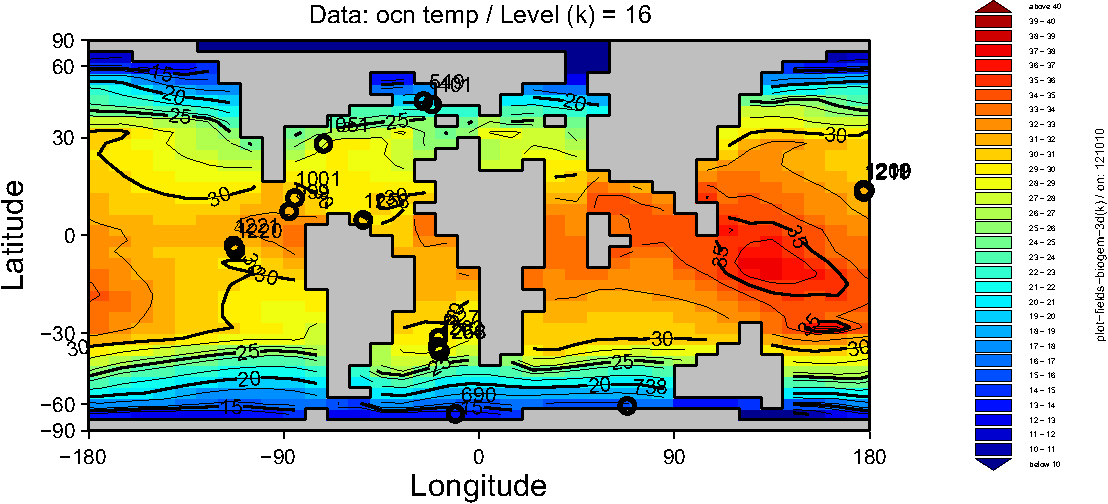
\includegraphics[scale=0.75]{cgenie_datalocations.pdf}
\end{center}
\caption{Paleocene-Eocene deep-sea sediment drill locations together with a contour-overlain map of surface temperature.}
\label{fig:cgenie_datalocations}
\end{figure}

%------------------------------------------------

\section{Sediment model output analysis}

%----------------------------------------------------------------------------------------
%----------------------------------------------------------------------------------------